\subsection{\LaTeX Examples}

This section should not be included in the final document.

I (Anders) have defined a macro for the project name. I have chosen
\epns{} for the reasons I give in the introduction.
The name can easily be changed by changing the macro\\
\textbackslash newcommand\{epns\}\{The name of our project\}\\
use \textbackslash epns\{\} to insert the name in your text.

\begin{figure}
\begin{center}
\begin{petri}
    \node at (0, 0) [place] (track) {};
	\node at (3, 2) [inputplace] (semaphore) {};
	\node at (3, 0) [transition] (connection) {};
	\node at (0, 0) [token] {};
	\draw [->,arc] (track) to [out=30,in=150] (connection);
	\draw [->,arc] (connection) to [out=210,in=330] (track);
	\draw [->,arc] (semaphore) -- (connection);
\end{petri}
\caption{Petri net model}
\label{fig:petri-model}
\end{center}
\end{figure}

\begin{figure}
\begin{center}
\begin{petri}[Very][Simple]
	\node at (2, 5) [place] (red) {};
	\node at (2, 2) [place] (green) {};
	\node at (2, 3.5) [inputplace] (input) {};
	\node at (0.5, 3.5) [transition] (turn green) {};
	\node at (3.5, 3.5) [transition] (turn red) {};
	\node at (2, 0) [transition] (connection) {};
	\node at (2, 2) [token] {};
	\draw [->,arc] (red) to [out=180,in=90] (turn green);
	\draw [->,arc] (green) to [out=0,in=270] (turn red);
	\draw [->,arc] (turn green) to [out=270,in=180] (green);
	\draw [->,arc] (turn red) to [out=90,in=0] (red);
	\draw [->,arc] (input) to [out=0,in=180] (turn red);
	\draw [->,arc] (input) to [out=180,in=0] (turn green);
	
	\draw [->,arc] (connection) to [out=75,in=285] (green);
	\draw [->,arc] (green) to [out=255,in=105] (connection);
	\draw [->,track arc] (0,0) -- (connection);
	\draw [->,track arc] (connection) -- (4,0);
\end{petri}
\caption{Petri net for a semaphore}
\label{fig:petri-semaphore}
\end{center}
\end{figure}

\begin{figure}
\begin{center}
\begin{petri}
	\node at (2, 5) [place] (left) {};
	\node at (2, 2) [place] (right) {};
	\node at (2, 3.5) [inputplace] (input) {};
	\node at (0.5, 3.5) [transition] (turn right) {};
	\node at (3.5, 3.5) [transition] (turn left) {};
	\node at (2, 0) [transition] (go right) {};
	\node at (2, 7) [transition] (go left) {};
	\node at (-2, 3.5) [track place] (incoming track) {};
	\node at (2, 2) [token] {};
	\node at (-2, 3.5) [train token] {};
	\draw [->,arc] (left) to [out=180,in=90] (turn right);
	\draw [->,arc] (right) to [out=0,in=270] (turn left);
	\draw [->,arc] (turn right) to [out=270,in=180] (right);
	\draw [->,arc] (turn left) to [out=90,in=0] (left);
	\draw [->,arc] (input) to [out=0,in=180] (turn left);
	\draw [->,arc] (input) to [out=180,in=0] (turn right);
	
	\draw [->,arc] (go right) to [out=75,in=285] (right);
	\draw [->,arc] (right) to [out=255,in=105] (go right);

	\draw [->,arc] (go left) to [out=255,in=105] (left);
	\draw [->,arc] (left) to [out=75,in=285] (go left);

	\draw [->,track arc] (incoming track) to [out=30,in=180] (go left);
	\draw [->,track arc] (incoming track) to [out=-30,in=180] (go right);
	\draw [->,track arc] (go right) -- (4,0);
	\draw [->,track arc] (go left) -- (4,7);
	\draw [->,track arc] (-4,3.5) -- (incoming track);
\end{petri}
\caption{Petri net for a switch}
\label{fig:petri-switch}
\end{center}
\end{figure}

In figure \ref{fig:petri-model} and the following figures are shown vector graphics of Petri nets 
created with Ti\textit{k}Z. Please see

\texttt{http://cremeronline.com/LaTeX/minimaltikz.pdf} for a short introduction



See \texttt{http://en.wikibooks.org/wiki/LaTeX/Indexing} for information on creating index entries

And here for an example of a figure, it is referenced with number \ref{fig:under-the-hood}:
\begin{figure}[htp]
\begin{center}
  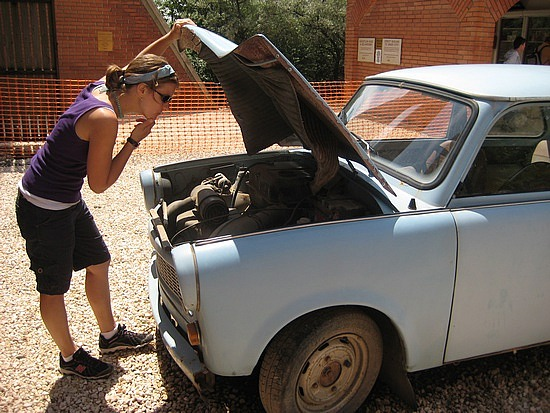
\includegraphics[width=10.0cm]{image/under-the-hood.jpg}
  \caption{Tja\ldots (Danish word \smiley)}
  \label{fig:under-the-hood}
\end{center}
\end{figure}

 

